\section{Preliminary insights}
Communities like Suicide watch are crucial for mental health awareness and mitigation efforts as they provide users suffering from mental health issues, an anonymous and safe way to discuss and vent out.
Particularly Suicide watch community consists of over 78k subscribers and reader, however is supported by mere 12 Moderators according to last count. These moderators are volunteers and do have a training, albeit through experience. All the moderators have been in that role for at least 3 years and the oldest goes as far as December 2008. 

As such it is valuable to understand how is a community like r/SuicideWatch thriving and in what aspects is this community similar or dis-similar from other casual subreddits. 

\subsection{Thread Engagement}
One thing to measure conversation was by difference or similarities in engagement with a thread in Subreddits. We look at two prime metrics, 1) Distribution of unique participants in a particular thread  2) Maximum Depth of a branch in the Reply graph of the thread . 
Figure \ref{fig:depthDist} shows the distribution of maximum depths across all Reply graphs for SW and AS subreddits. The SW theads depths have a median depth of 5 and mean of 7.5 compared to a median depth of 1 and mean of 1.7 for AS subreddits. This shows that on an average the longest branch of reply graphs for SW subreddits are much longer than the baseline subreddit. This is despite the fact that AskScience has a two order of magnitude advantage in terms of subscribed users (14,999,331) over Suicide watch(78,000). 
\begin{figure}[!h]
	\centering
	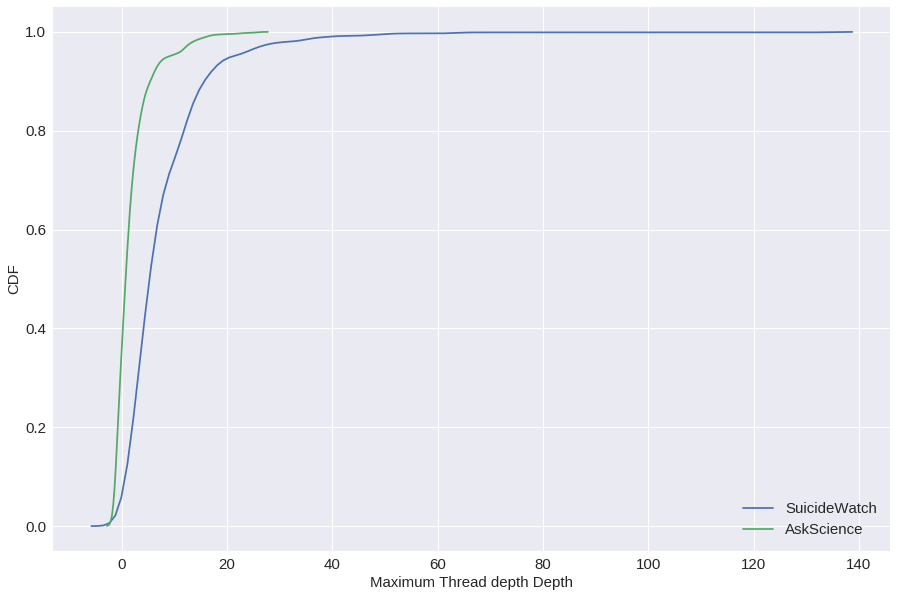
\includegraphics[width=0.5\columnwidth]{Figures/depthDist}
	\caption{\textsl{ Distribution of maximum depth of Reply Graphs for Subreddits r/SuicideWatch and r/AskScience }}
	\label{fig:depthDist}
\end{figure}

However if we  compare the number of unique users per thread, the two communities do not exibit much difference. SW subreddit has a median of 6 users per thread and a mean of 6.7 users and AS subreddit has a median of 5 users and mean of 13.3 users. So this shows than there is a somewhat uniform participation in terms of unique users responding to $RP$ on SW and a skewed but still at par participation on AS. 
% \begin{figure}[!h]
% 	\centering
% 	\includegraphics[width=\columnwidth]{Figures/userDist}
% 	\caption{\textsl{ Distribution of maximum depth of Reply Graphs for Subreddits r/SuicideWatch and r/AskScience }}
% 	\label{fig:userDist}
% \end{figure}

\subsection{Network structure}
Because of the networked abstraction of threads as described in Sec \ref{Sec:Conversations}, we can now compare subreddits using network structural properties like degree distribution and structural holes in terms of conversations. 
Figures \ref{fig:repDegreeDist} and \ref{fig:userDegreeDist} show the comparison of degree distributions for both user and Reply graphs for two distinct sub-reddits. Despite having differences in terms of conversation depth, these two communities look similar in terms of classical degree distribution metrics. 

\begin{figure}[!ht]
	\centering
	% \hspace*{-5mm}
	\subfloat[]{
		\includegraphics[width=0.45\textwidth, height = 5cm ]{Figures/degreeDist}
		\label{fig:rGraphSW}
	}
	\subfloat[]{
		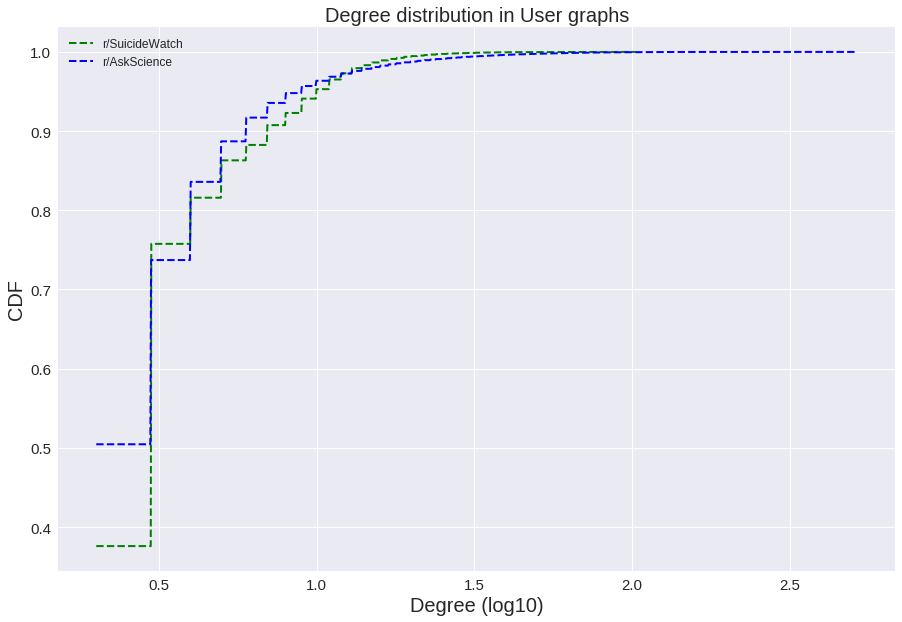
\includegraphics[width=0.45\linewidth, height = 5cm ]{Figures/degreeDistUgraph}
		\label{fig:uGraphSW}
	}
\caption{Fig \ref{fig:rGraphSW} shows Distribution of degrees for Reply Graphs,  r/SuicideWatch and FrontPage. Fig \ref{fig:uGraphSW} shows the degree distributions for the reply graphs}
\end{figure}

To compare the extent of similarity, we use the Mann-Whitey-U test. We calculate the test statistic across two sampled set of graphs taken from dataset of user and reply graphs for the baseline and SW subreddits. We then compare the cross dataset statistic with the statistic calculated between samples taken from the same dataset. This gives us an idea about similarity between two datasets. What we found that the distribution of degress for User and Reply graphs for SW and AS subreddits is up to 85\%. 

\subsection{Response Times}
Understanding the inter message times can act as a good proxy for the urgency in a conversation. To understand how Suicide watch subreddit users responds to a $OP$ compared to other sub-reddits like r/AskScience, we calculate differences between the posting times between consecutive messages in a reply graph. Figure \ref{fig:responseTimeDist} shows comparison using CDFs of inter-message response times for SW and AS subreddits. It can be seen that SW $OP$ are responded with the higher urgency compared to either the $OP$ or any other user for AS sub-reddits. 

\begin{figure}[!h]
	\centering
	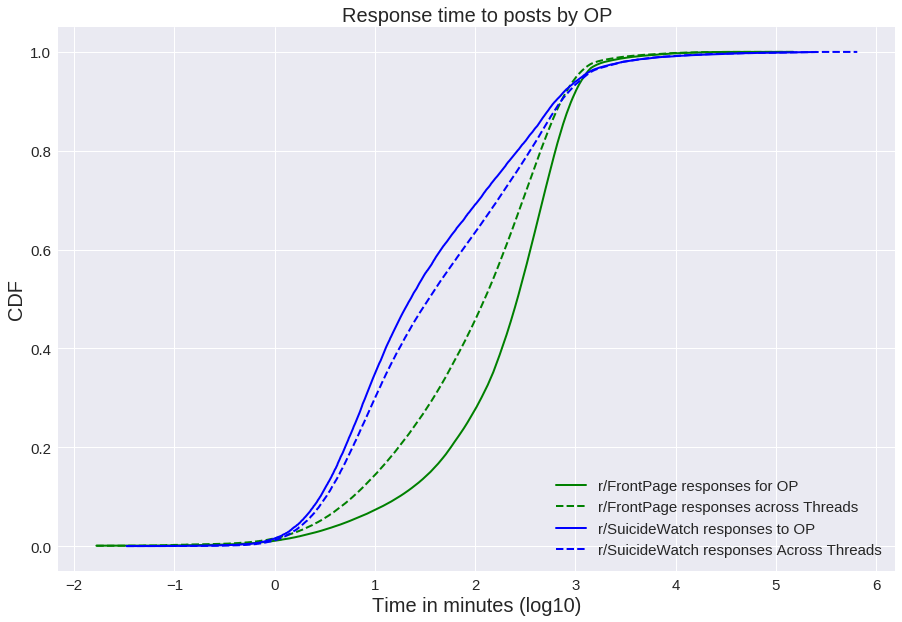
\includegraphics[width=0.5\columnwidth]{Figures/respTimeDist}
	\caption{\textsl{ Distribution of degrees for User Graphs,  r/SuicideWatch and r/AskScience }}
	\label{fig:responseTimeDist}
\end{figure}

\subsection{Symmetric responses}
Despite signs of urgency and engagement, we ask the question: what percentage of conversations happening on these subreddits are symmetric in nature ? 
For this we first define a Symmetric user and a symmetric message. For a user $V_i$ in the user graph $G\{V,E,W\}$ as described in Section \ref{Sec:Conversations} , a symmetric user is a user who interacts with $V_o$ or the $OP$ and receives a response from the $OP$. We find the fraction $$U_{sym}=\frac{\textit{total number of symmetric users }}{\textit{Total users in a thread}}$$
Figure \ref{fig:symUsers} shows the CDF of $U_{sym}$ across the SW and AS sub-redditor.  The median value for $U_{sym}$ for SW is 20\% where as for AS is 0\%. This shows that SW subreddit engages is a lot more symmetric conversation that the baseline moderated subreddit like AS.

\begin{figure}[!ht]
	\centering
	% \hspace*{-5mm}
	\subfloat[]{
		\includegraphics[width=0.45\textwidth, height = 5cm ]{Figures/SymMessages_SW_FP}
		\label{fig:rGraphSW}
	}
	\subfloat[]{
		\includegraphics[width=0.45\linewidth, height = 5cm ]{Figures/SymmetricSW_FP}
		\label{fig:uGraphSW}
	}
\caption{Fig \ref{fig:rGraphSW} shows Distribution of degrees for Reply Graphs,  r/SuicideWatch and FrontPage. Fig \ref{fig:uGraphSW} shows the degree distributions for the reply graphs}
\end{figure}


If we define a set of users who engage in symmetric activity with the $OP$ , it would be worth while to investigate how much of the total message activity on the thread is carried out by these set of symmetric users . To calculate this we find the fraction of messages on each thread written as part of this symmetric conversation. Figure \ref{fig:symMessages} shows the trend. It can be see that SW threads contain a higher prevalence of symmetric message exchanges compared to the baseline AS subreddit 

\subsection{Centralities}
To understand how embedded is the $OP$ in a conversation thread, we compare the betweenness centralities of $OPs$ in the $SW$ dataset with the baseline $FP$ dataset. 
Betweenness centralit of a node $v$ is defined as 
\begin{equation}
	g(v) = \sum_{s \neq v \neq t}\frac{\sigma_{st}(v)}{\sigma_{st}}
\end{equation}
where $\sigma_{st}(v)$ is the total number of shortest paths from node $s$ to node $t$ and $\sigma_{st}$ is the number of those paths that pass through $v$.
\begin{figure}[!h]
	\centering
	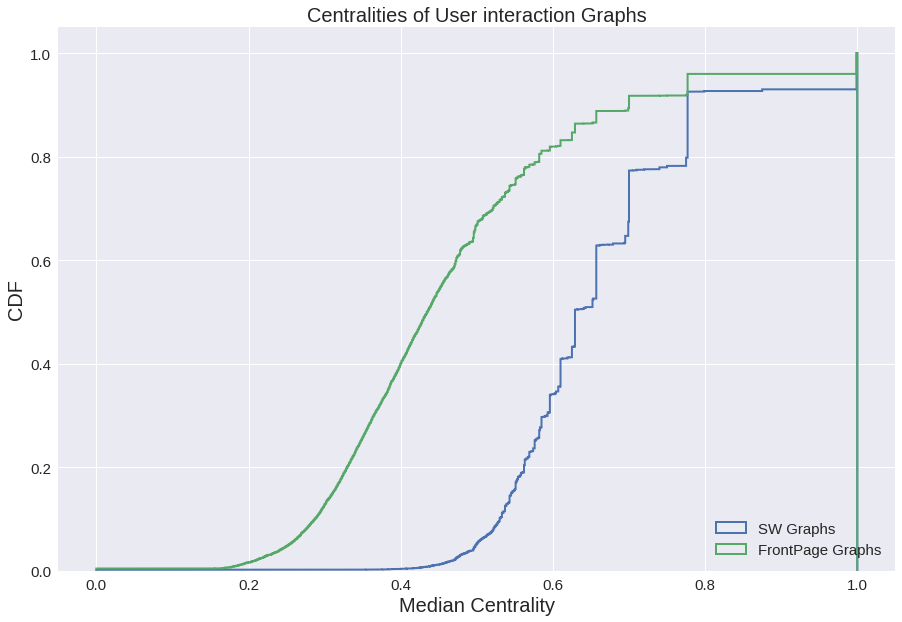
\includegraphics[width=0.5\columnwidth]{Figures/Betweenness_SW_FP}
	\caption{\textsl{ CDF for Betweenness Centralities of $OP$ compared to random threads from the Reddit $FP$ }}
	\label{fig:centralities}
\end{figure}
Betweenness centrality is a good proxy of understanding how closely linked is a node with the rest of the network. When we calculate this metric for the user graphs we see that Suicide watch $OPs$ tend to have higher centralities compared to generic $FP$ threads. 